% !TEX root =  ../Dissertation.tex

\chapter{Project Management}

The timeline of the project can be seen in the below Gantt chart
\cref{fig:Gantt}. The focus on the first 2 months was to write Agda Tree and
Agda Comp. For Agda Tree, the first milestone was to parse an Agda project and to
extract the definition dependency graph. The next milestone is to implement the
queries on the dependency graph. Once the queries were implemented,
the last milestone was the Command Line Interface that gives the user a
way to run those queries with their own parameters. Lastly, the queries were
unit tested for correctness and for performance. This was done by the
date of the demonstration, which is a major milestone as it marked the first
stable version of the CLI tools.

While developing Agda Tree, Agda Comp was also being developed. The first task
of Agda Comp was to explore different compilation strategies and different
methods to compile an Agda project. Once the strategies were selected, they
were tested for correctness, safety and compilation time which was a major
milestone. With the strategies implemented, the CLI was created that
runs the strategy and compilation strategy. This was done by the date
of the demonstration.

An agile software development methodology was used, as seen by the time-line
there are multiple tasks running at the same time until they are all completed
by the demonstration. There were weekly meetings with my supervisor were a
working state of the project was shown along with a summary of all the
accomplishments since the previous week, and my supervisor gives suggestions on
improvements and additions for next week. This iterative approach allowed for
a skeleton of the tools to be quickly created for my supervisor to test.

\begin{figure}[H]
    \centering
    \label{fig:Gantt}
    \makebox[\textwidth]{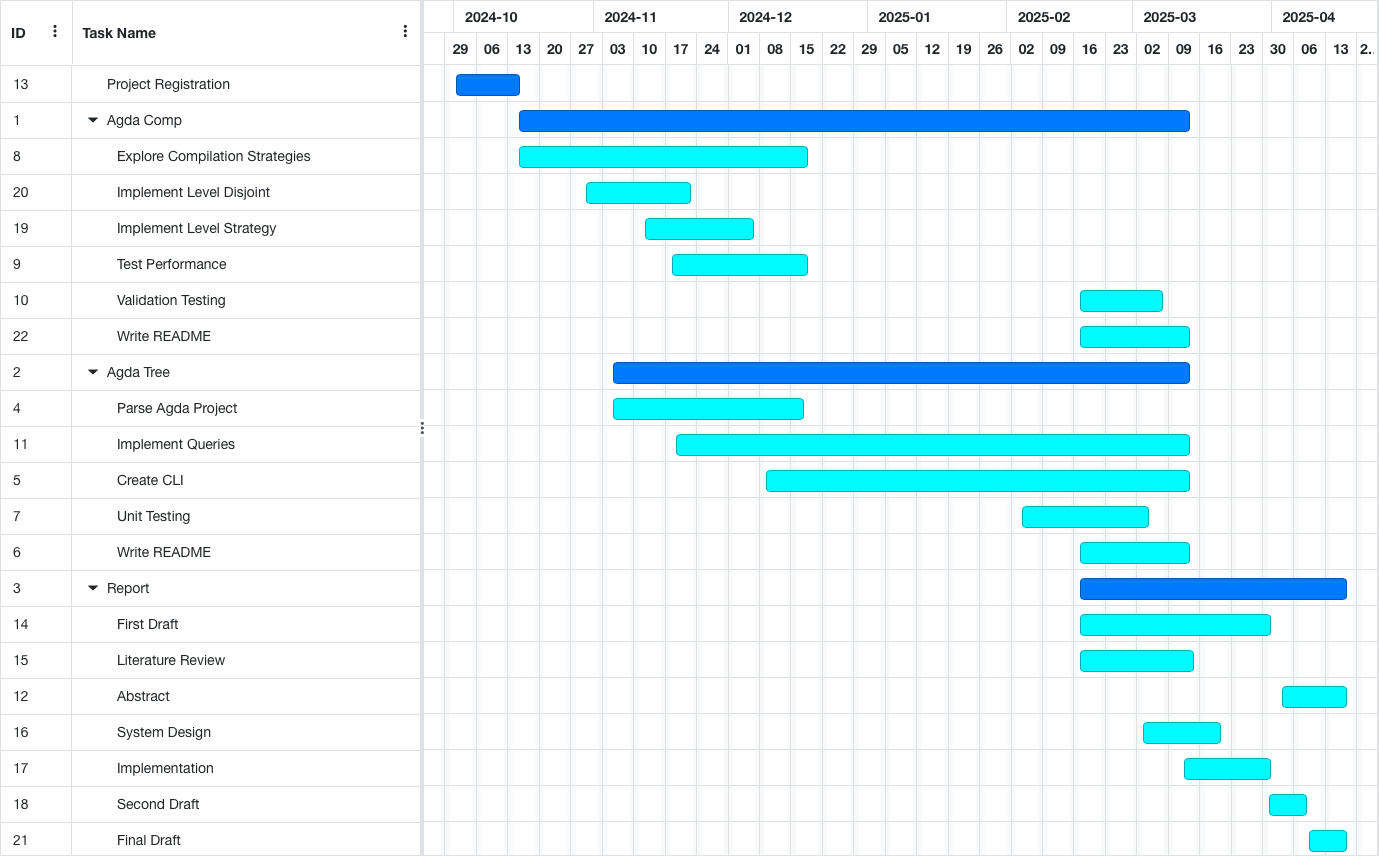
\includegraphics[width=\textwidth]{Gantt.png}}
    \caption{Gantt Chart}
\end{figure} 


% What is the timeline for your project? What software development
% methodology will you use? Can you identify the major milestones? These types of questions are
% important for project planning and should be addressed directly.
%
% \begin{itemize}
% \item Gantt chart 
% \item Weekly updates with supervisor 
% \item Getting the s-expression extractor was a major milestone 
% \item Using python instead of clojure was a significant improvement
% \end{itemize}
%
% | Week | Goal | Outcome |
% | ------------- | -------------- | -------------- |
% | S1.Wk1 <br> 30th September 2024  | Pick Project idea and analyze HTML files and explore what data can be accessed | Chose project idea, analysing agda HTML files for easier searching and created python script that reads Agda HTML files and returns all of the found symbols |
% | S1.Wk2 | Complete project registration and research related works | Registered project and learned about LSPs and Ctags but they don't quite match our use case. |
% | S1.Wk3 | Research and implement graphs |  |
% | S1.Wk4 | Implement some queries | |
% | S1.Wk5 | Implement some queries | |
% | S1.Wk6 | Implement some queries | |
% | S1.Wk7 | Implement some queries | |
% | S1.Wk8 | Implement some queries | |
% | S1.Wk9 | Implement some queries | |
% | S1.Wk10 |Test scalability | |
% | S1.Wk11 | Test scalability | |
% | CV1 | | |
% | CV2 | | |
% | CV3 | | |
% | CV4 | | |
% | S1.Wk12 | Write Introduction | |
% | S2.Wk1 | Write Literature review | |
% | S2.Wk2 | Write Legal/Social/Ethica issues | |
% | S2.Wk3 | Write requirements | |
% | S2.Wk4 | Write Design of the software | |
% | S2.Wk5 | Write how I implemented the software | |
% | S2.Wk6 | Write testing and success Measurement | |
% | S2.Wk7 | Write Project Management | |
% | S2.Wk8 | Write Evaluation | |
% | S2.Wk9 | Proof read | |
% | S2.Wk10 | Proof read | |
% | S2.Wk11 | Write abstract | |
% | EV1 | Proof read | |
% | EV2<br>  5pm on 17th April 2025 | | |
